% =====================================================================
% Recurrent linear-optical reservoir computing.
% Tables come from results_tables.tex, generated by
%   python scripts/make_paper_tables.py
% Figures come from results/figures/, generated by
%   python experiments/make_figures.py
% Do not type result numbers by hand.
% =====================================================================
\documentclass[11pt]{article}

\usepackage[utf8]{inputenc}
\usepackage[T1]{fontenc}
\usepackage{lmodern}
\usepackage{amsmath, amssymb, amsthm}
\usepackage{siunitx}
\usepackage{booktabs}
\usepackage{multirow}
\usepackage{graphicx}
\usepackage{float}
\usepackage{placeins}
\usepackage[dvipsnames]{xcolor}
\usepackage{hyperref}
\usepackage[round, authoryear]{natbib}
\usepackage{microtype}
\usepackage{geometry}
\geometry{margin=1in}

\graphicspath{{../../results/figures/}}
% Generated by scripts/make_paper_tables.py -- do not edit by hand.
% Regenerate after any results change:  python scripts/make_paper_tables.py
% Requires siunitx for \num.

\newcommand{\PaperTableBenchmarks}{%
\begin{tabular}{lrrrrrr}
\toprule
Model & NARMA-5 & NARMA-10 & NARMA-20 & Mackey-Glass ($h{=}17$) & Lorenz-63 ($h{=}20$) & S\&P 500 RV \\
\midrule
Photonic (recurrent) & 0.0152 (0.0043) & \textbf{0.0951 (0.0168)} & \textbf{0.2409 (0.0456)} & \textbf{0.0005 (0.0005)} & 0.2810 (0.1638) & 0.6993 (0.0015) \\
Photonic (no feedback) & 0.0152 (0.0043) & 0.2156 (0.0322) & 0.4355 (0.1280) & 0.0005 (0.0005) & 0.2821 (0.1365) & 0.6993 (0.0015) \\
Echo state network & \textbf{0.0109 (0.0023)} & 0.2794 (0.1108) & 0.4132 (0.1119) & 0.0005 (0.0002) & 0.3396 (0.7024) & \textbf{0.6823 (0.0014)} \\
Random Fourier features & 0.0164 (0.0023) & 0.1759 (0.0538) & 0.4347 (0.0821) & 0.0014 (0.0016) & \textbf{0.2110 (0.5884)} & 0.7274 (0.0135) \\
Polynomial window & 0.0158 (0.0033) & 0.1763 (0.0460) & 0.4741 (0.1844) & 0.0204 (0.0146) & 3.3614 (2.6976) & 0.7045 (0.0000) \\
Linear window (control) & 0.3801 (0.0450) & 0.4446 (0.0904) & 0.4495 (0.0969) & 0.6176 (0.0592) & 0.9187 (0.0376) & 0.6957 (0.0000) \\
\bottomrule
\end{tabular}
}

\newcommand{\PaperTableDM}{%
\begin{tabular}{lrrrrrr}
\toprule
Baseline vs photonic & NARMA-5 & NARMA-10 & NARMA-20 & Mackey-Glass ($h{=}17$) & Lorenz-63 ($h{=}20$) & S\&P 500 RV \\
\midrule
Photonic (no feedback) & 1.0000 & 0.0002 & 0.0000 & 1.0000 & 0.4788 & 1.0000 \\
Echo state network & 0.0572 & 0.0000 & 0.0000 & 0.4062 & 0.0248 & 0.4451 \\
Random Fourier features & 0.3226 & 0.0002 & 0.0000 & 0.0004 & 0.9599 & 0.2880 \\
Polynomial window & 0.1876 & 0.0001 & 0.0000 & 0.0002 & 0.0034 & 0.7888 \\
Linear window (control) & 0.0000 & 0.0000 & 0.0000 & 0.0000 & 0.0000 & 0.8776 \\
\bottomrule
\end{tabular}
}

\newcommand{\PaperTableCapacity}{%
\begin{tabular}{lrr}
\toprule
Model & Feature dim. & NRMSE \\
\midrule
Photonic (recurrent) & 1381 & 0.1092 $\pm$ 0.0369 \\
Photonic (recurrent) & 701 & 0.1643 $\pm$ 0.0156 \\
Random Fourier features & 1200 & 0.1876 $\pm$ 0.0604 \\
Random Fourier features & 600 & 0.2373 $\pm$ 0.0631 \\
Echo state network & 501 & 0.2660 $\pm$ 0.0402 \\
Echo state network & 1001 & 0.2676 $\pm$ 0.0920 \\
Polynomial window & 679 & 0.4566 $\pm$ 0.0488 \\
\bottomrule
\end{tabular}
}

\newcommand{\PaperTableMemory}{%
\begin{tabular}{lrrrr}
\toprule
System & Dim. & Linear MC & IPC & IPC/feature \\
\midrule
photonic no feedback & 132 & 10.5 & 111.9 & 0.85 \\
linear window 20 & 20 & 19.1 & 13.0 & 0.65 \\
esn 200 & 201 & 27.0 & 123.9 & 0.62 \\
photonic & 132 & 11.1 & 69.3 & 0.52 \\
esn 500 & 501 & 29.6 & 213.9 & 0.43 \\
\bottomrule
\end{tabular}
}

\newcommand{\PaperTableNoise}{%
\begin{tabular}{rr}
\toprule
Coincidences/step & NRMSE \\
\midrule
$\infty$ & 0.2748 $\pm$ 0.0279 \\
30 & 0.4901 $\pm$ 0.0354 \\
100 & 0.5340 $\pm$ 0.0520 \\
300 & 0.4626 $\pm$ 0.0192 \\
1000 & 0.4113 $\pm$ 0.0439 \\
3000 & 0.4038 $\pm$ 0.0480 \\
10000 & 0.3798 $\pm$ 0.0153 \\
30000 & 0.3433 $\pm$ 0.0303 \\
\bottomrule
\end{tabular}\hfill
\begin{tabular}{rr}
\toprule
Indistinguishability & NRMSE \\
\midrule
0.5 & 0.2484 \\
0.6 & 0.2482 \\
0.7 & 0.2483 \\
0.8 & 0.2468 \\
0.85 & 0.2478 \\
0.9 & 0.2486 \\
0.95 & 0.2483 \\
1 & 0.2479 \\
\bottomrule
\end{tabular}\hfill
\begin{tabular}{rr}
\toprule
$g^{(2)}(0)$ & NRMSE \\
\midrule
0 & 0.2479 \\
0.02 & 0.2480 \\
0.05 & 0.2482 \\
0.1 & 0.2485 \\
0.2 & 0.2492 \\
0.3 & 0.2498 \\
\bottomrule
\end{tabular}
}

\newcommand{\PaperTableRates}{%
\begin{tabular}{lrrr}
\toprule
Platform & $n$ & Coincidences/s & Time for $3\times10^4$ \\
\midrule
Ascella & 2 & \num{4.76e+04} & 0.63\,s \\
Ascella & 3 & \num{1.16e+03} & 25.81\,s \\
Ascella & 4 & \num{2.84e+01} & 18\,min \\
Belenos & 2 & \num{1.16e+04} & 2.59\,s \\
Belenos & 3 & \num{5.60e+02} & 53.56\,s \\
Belenos & 4 & \num{2.71e+01} & 18\,min \\
\bottomrule
\end{tabular}
}



\title{A Recurrent Linear-Optical Reservoir for Time-Series Forecasting:\\
       Matched-Capacity Benchmarks and Robustness at Measured\\
       Photonic-Hardware Noise Levels}

\author{%
  H\"useyin Umut I\c{s}\i{}k\textsuperscript{1,*},\,
  Arda Kara\textsuperscript{2,*},\,
  Mehmet Alp \"Ozayd\i{}n\textsuperscript{1},\,
  Eren Aslan\textsuperscript{1}
  \\[0.6em]
  \normalsize \textsuperscript{1}Middle East Technical University, Ankara, Turkey \\
  \normalsize \textsuperscript{2}Bilkent University, Ankara, Turkey \\
  \normalsize \textsuperscript{*}Co-first authors; equal contribution.
}
\date{\today}

\begin{document}
\maketitle

\begin{abstract}
We study a linear-optical reservoir computer in which a leaky-integrated state is fed back
into the phase encoding of a fixed photonic interferometer, with only a ridge readout
trained. The feedback is applied classically between measurement batches, so the recurrent
model consumes exactly the same shot budget as a memoryless windowed encoding and requires
no optical memory or fast feed-forward. Evaluated under the standard input-driven
reservoir-computing protocol, the model attains median NRMSE $0.095$ on NARMA-10 and
$0.241$ on NARMA-20, outperforming a tuned echo state network, random Fourier
features, a polynomial expansion of the input window, and a linear control, with
Diebold--Mariano $p < 0.001$ against every baseline. Because the tuned configuration uses
more features than the baselines, we sweep every model family across a common feature
dimension: at $\approx 1400$ features the photonic map attains $0.109$ against $0.188$ for
random Fourier features and $0.268$ for an echo state network, and the latter saturates
beyond $2000$ units while the photonic map does not. Removing the feedback, with all else
fixed, doubles the error on both NARMA tasks. It ties a tuned echo state network on
Mackey--Glass; loses to one on NARMA-5 --- a task needing only five steps of memory, where
long linear memory suffices and the photonic map's nonlinearity buys nothing; loses to random
Fourier features on Lorenz-63, where per-seed errors span two orders of magnitude and five
seeds cannot separate the candidates; and ranks third of six on S\&P~500 realised volatility
with no model statistically distinguishable from any other. Every outcome is reported
unmodified.
Simulating the Ascella and Belenos operating points read from Quandela's cloud API with
threshold detectors, we find accuracy essentially unchanged by photon distinguishability
(flat for Hong--Ou--Mandel visibility from $0.50$ to $1.00$) and by multi-photon emission
($+0.8\%$ for $g^{(2)}(0)$ from $0$ to $0.30$), while finite sampling dominates. Since
$n$-fold coincidence rate falls as $\eta^{n}$ in the transmittance $\eta$, this inverts the
usual design instinct: photon number, not photon quality, is the binding constraint. Testing
that directly, we find no detectable benefit from photon indistinguishability on seven of eight
task and photon-number configurations, so we conclude that the architecture is a classical
random nonlinear feature map realised in optics and that the exploited resource is Fock-space
dimension rather than interference. Comparing measured classical throughput against measured
device rates, no crossover with simulation exists at any photon number on current hardware; a
crossover at twelve photons in twenty-four modes would require roughly a fourfold improvement
in transmittance. We make no claim of quantum advantage, and all results reported here are
simulated.
\end{abstract}

\section{Introduction}\label{sec:intro}

Reservoir computing trains only a linear readout on the state of a fixed nonlinear dynamical
system \citep{jaeger2001esn, maass2002lsm}. Photonic implementations are attractive because a
passive interferometer realises a high-dimensional nonlinear map at no energetic cost per
inference, and because boson sampling supplies a feature space whose dimension grows
combinatorially with photon and mode number \citep{garciabeni2023scalable,
nerenberg2025photonquarc}. Recent work has demonstrated quantum optical reservoirs on
Quandela's Ascella processor \citep{maring2024ascella} and applied related architectures to
financial forecasting \citep{amanov2026hpqrc, li2025qrcrv}.

Two questions decide whether such a system is worth building, and the literature answers
neither cleanly. First, does the optical feature map do anything a cheap classical feature map
does not, at matched feature dimension and against baselines tuned with equal budget? Second,
does it survive the noise of an actual device --- and if not, which noise source is
responsible?

This paper addresses both. Our contributions:

\begin{itemize}
  \item \textbf{A recurrent formulation whose feedback is free on hardware.} The reservoir
        state is fed back into the encoding phases and integrated with a leak rate
        (Section~\ref{sec:method}). Because the feedback is computed classically between
        measurement batches, each timestep remains a single circuit configuration and a
        single batch of samples. The recurrent model therefore costs the same number of shots
        as a stateless windowed encoding.
  \item \textbf{Matched-capacity benchmarking.} We sweep every model family across a common
        feature-dimension range rather than comparing tuned configurations of different size
        (Section~\ref{sec:capacity}).
  \item \textbf{An architectural prediction that the data confirms.} NARMA-$N$ contains the
        cross-lag product $u_t u_{t-N+1}$, which a linear-optical map can only form if both
        lags occupy the same encoding. The optimal encoding window tracks the task order
        (Section~\ref{sec:encoding}).
  \item \textbf{A noise study at measured device parameters} showing that accuracy is
        insensitive to distinguishability and multi-photon emission but strongly limited by
        coincidence count, yielding a concrete feasibility threshold
        (Section~\ref{sec:noise}).
  \item \textbf{A direct test of whether interference contributes}, by interpolating between
        distinguishable and indistinguishable photons at otherwise identical settings. It does
        not, on seven of eight configurations, so we characterise the architecture as a
        classical random nonlinear feature map realised in optics and identify Fock-space
        dimension as the exploited resource (Section~\ref{sec:quantumness}).
  \item \textbf{A crossover analysis} against the measured cost of simulating the same map,
        which finds no crossover on current hardware and quantifies the transmittance a
        crossover would require (Section~\ref{sec:crossover}).
\end{itemize}

We also report, in Section~\ref{sec:limitations}, that an earlier windowed version of this
architecture did not outperform a ridge regression on the raw input window, and why.

\section{Background and related work}\label{sec:background}

An echo state network maintains $x_t = (1-a)x_{t-1} + a\tanh(W_{\text{in}}[1;u_t] + Wx_{t-1})$
with $W$ scaled to a chosen spectral radius, and fits a linear readout on $x_t$
\citep{jaeger2001esn}. Its capacity is characterised by linear memory capacity
\citep{jaeger2001esn} and, more completely, by information processing capacity over an
orthogonal basis of nonlinear functionals of the input history \citep{dambre2012ipc}.

Quantum optical reservoirs replace the recurrent tanh map with the output distribution of a
linear interferometer over Fock space \citep{garciabeni2023scalable, nerenberg2025photonquarc}.
For $n$ indistinguishable photons in $m$ modes injected one per input mode, the amplitude for
a collision-free output pattern $S$ is the permanent of the submatrix $U[S,T]$, with $T$ the
input modes, so the accessible feature dimension is $\binom{m}{n}$. We simulate this exactly
using Perceval \citep{heurtel2023perceval}.

The closest prior work applies photonic or Ising quantum reservoirs to financial series
\citep{amanov2026hpqrc, li2025qrcrv}; \citet{branco2024hardtobeat} and \citet{bienstman2025nalm}
argue that such comparisons frequently omit the classical control that would make them
informative. We take that objection seriously enough to place a linear ridge on the raw input
window in every table.

\section{Method}\label{sec:method}

\subsection{Reservoir dynamics}

Let $u_t \in \mathbb{R}^{d}$ be the driving input. Write $\tilde{u}_t$ for the concatenation of
the most recent $k$ lags of $u$, where $k$ is the \emph{encoding window}. The reservoir keeps a
state $s_t \in \mathbb{R}^{P}$, $P = \binom{m}{n}$, and evolves as
\begin{align}
  e_t &= g_{\text{in}} W_{\text{in}} \tilde{u}_t
       + g_{\text{fb}} W_{\text{fb}}\!\left(P s_{t-1} - \mathbf{1}\right) + b, \label{eq:encode}\\
  p_t &= \operatorname{BosonSample}\!\left(U(e_t)\right), \label{eq:optics}\\
  s_t &= (1-\lambda)\, s_{t-1} + \lambda\, p_t. \label{eq:leak}
\end{align}
Here $e_t$ are phase-shifter settings in radians, $U(e_t)$ is the resulting circuit unitary,
and $p_t$ is the distribution over collision-free outputs. The matrices $W_{\text{in}}$,
$W_{\text{fb}}$, the bias $b$ and the interferometer are fixed random draws and are never
trained; only a ridge readout on $[s_t, \text{input window}]$ is fitted.

Two details matter. The state is fed back as $Ps_{t-1}-\mathbf{1}$, its deviation from the
uniform distribution, whose entries are $O(1)$ regardless of Fock-space size; with
$W_{\text{fb}}$ drawn at variance $1/P$, the gain $g_{\text{fb}}$ then means the same thing at
every photon number, so a photon-number ablation does not silently confound expressivity with
feedback strength. And the gains $g_{\text{in}}, g_{\text{fb}}$ are free parameters rather than
implicit: a naive encoding that applies the raw series directly as phases uses only a small
fraction of the available $2\pi$ range, which we found to be the dominant failure mode of the
predecessor architecture (Section~\ref{sec:limitations}).

\subsection{Feedback is classical and therefore free}\label{sec:free-feedback}

Equation~\eqref{eq:leak} is evaluated on measured probabilities, on a classical computer,
between measurement batches. Each timestep is still one circuit configuration and one batch of
samples. A recurrent run therefore requires exactly as many shots as a stateless one --- the
recurrence adds no photonic resource whatsoever. This is what makes the architecture
deployable on current cloud-accessed hardware, where a closed optical feedback loop is not
available.

The corresponding cost is a scheduling one: step $t$'s phases depend on step $t-1$'s
measurement, so the timesteps of a closed loop cannot be batched into a single cloud job. We
return to this in Section~\ref{sec:hardware}.

\subsection{Exact simulation}\label{sec:core}

The circuits used here are layered,
$U = A_d D(\phi_{d-1}) A_{d-1} \cdots A_1 D(\phi_0) A_0$, with the $A_k$ fixed and $D(\phi)$ a
diagonal layer of encoded phases. We therefore build the $A_k$ once and evaluate each timestep
as a few $m \times m$ products followed by a batch of $n \times n$ permanents. This agrees with
MerLin and with Perceval's SLOS backend to $10^{-16}$ while being $\sim$310$\times$ faster per
step, which is what makes a sequential recurrent loop affordable across seeds and
hyperparameter searches.

\subsection{Evaluation protocol}\label{sec:protocol}

All models pass through an identical pipeline. One continuous series is split into
washout / train / validation / test. The reservoir state is carried across split boundaries:
the reservoir has no trained parameters, so driving it over later data is not leakage, and
restarting the state at the test boundary would penalise exactly the memory under study. Every
quantity fitted from data --- input scaler, feature scaler, ridge penalty and readout --- is
estimated on training rows only.

The ridge penalty is selected on the validation slice \emph{per model}. This matters: a single
shared penalty favours whichever feature count it happens to suit, across models whose
dimensions differ by an order of magnitude.

We report NRMSE, the root mean squared error divided by the standard deviation of the target,
as used in the reservoir-computing literature. Inference uses Diebold--Mariano
\citep{diebold1995dm} with Newey--West HAC variance \citep{newey1987hac, andrews1991bandwidth}
and the Hansen Model Confidence Set \citep{hansen2011mcs} with a stationary bootstrap
\citep{politis1994stationary}.

\subsection{Baselines}\label{sec:baselines}

Every baseline receives the same Optuna trial budget as the photonic model.

\begin{itemize}
  \item \textbf{Linear window (control)}: ridge on a window of the raw drive. This is the
        model any claim about optical features must clear.
  \item \textbf{Echo state network} with input scaling, leak rate, spectral radius and
        sparsity all tuned. We note that omitting the input-scaling parameter --- as a
        surprising amount of code does --- costs roughly a factor of three on NARMA-10 and
        makes the baseline far too easy to beat.
  \item \textbf{Random Fourier features} \citep{rahimi2007rff} on the input window, the
        matched-dimension random nonlinear feature map.
  \item \textbf{Polynomial window}: explicit monomials up to degree three. NARMA targets are
        polynomial in the drive, so this bounds how much of any gain is simply ``some
        nonlinearity in the window''.
  \item \textbf{Photonic without feedback}: the identical optical map with recurrence
        disabled.
\end{itemize}

\section{Experiments}\label{sec:experiments}

Tasks span three distinct sources of temporal difficulty. NARMA-5, NARMA-10 and NARMA-20
\citep{jaeger2001esn} are driven by i.i.d.\ uniform input and demand nonlinear memory of a
stochastic drive. Mackey--Glass at horizon 17 is delay-induced chaos. Lorenz-63 at horizon 20
is deterministic continuous-time chaos, probing how far ahead a model can forecast before
sensitive dependence destroys predictability. Monthly S\&P~500 realised volatility
\citep{corsi2009} is the one empirical series.

Horizon choice matters for the chaotic tasks and we set it deliberately. Lorenz-63 at horizon
1 discriminates nothing --- a tuned echo state network and a plain ridge both score
$\sim\!10^{-4}$, because at $\mathrm{d}t = 0.02$ the next sample is nearly a linear function
of the current one. Past horizon 80, NRMSE exceeds 1 for every model, meaning none beats
predicting the mean. Horizon 20, roughly $0.4$ Lyapunov times, is the window in which the
task separates models.

\subsection{Forecasting accuracy}\label{sec:accuracy}

\begin{table}[H]\centering
  \PaperTableBenchmarks
  \caption{NRMSE, median (interquartile range) over 5 seeds, standard input-driven protocol.
           Lower is better; best per column in bold. Medians rather than means because the
           seed distribution on the chaotic tasks is heavy-tailed: one unlucky Lorenz-63
           trajectory raises a model's mean to $3.5\times$ its median and would decide the
           ranking on a single draw.}
  \label{tab:benchmarks}
\end{table}

\begin{table}[H]\centering
  \PaperTableDM
  \caption{Diebold--Mariano $p$-values with Newey--West HAC variance, each baseline against
           the recurrent photonic model.}
  \label{tab:dm}
\end{table}

The photonic reservoir wins NARMA-10 and NARMA-20 with $p < 0.001$ against every baseline. On
Mackey--Glass it ties the echo state network ($p = 0.41$); the task saturates, with three
models at $5\!\cdot\!10^{-4}$. It wins where the task demands nonlinear memory of a stochastic
drive, and not elsewhere.

Three results run against it, and are worth stating explicitly. On \textbf{NARMA-5} the echo
state network wins. This is the expected place to lose: the task requires only five steps of
memory, precisely the regime where a large tanh reservoir's long linear memory is sufficient
and the photonic map's extra nonlinearity buys nothing --- the mirror image of
Section~\ref{sec:ipc}. On \textbf{Lorenz-63} random Fourier features win on the median; the
photonic model has the better \emph{mean}, but that ordering inverts under a single seed and
we do not claim it. Across models the per-seed NRMSE spans $0.06$ to $11.0$ on this task, and
five seeds cannot separate the candidates. On \textbf{S\&P~500 realised volatility} it ranks
third of six and no model is distinguishable from any other ($p = 0.45$--$0.88$); we draw no
conclusion from the financial task.

Removing feedback while changing nothing else roughly doubles the error on both NARMA tasks
($p < 0.001$), which is the ablation the architecture rests on.

The Model Confidence Set retains almost every model on every task. With 200--600 test points
it has little power here, and we report it for completeness rather than as a discriminating
test.

\subsection{Matched capacity}\label{sec:capacity}

The tuned photonic configuration uses more features than the baselines, so a direct comparison
of Table~\ref{tab:benchmarks} would confound the feature map with its size. We therefore sweep
each family across a common dimension range.

\begin{table}[H]\centering
  \PaperTableCapacity
  \caption{NARMA-10, feature dimensions between 500 and 1500, mean over 3 seeds.}
  \label{tab:capacity}
\end{table}

\begin{figure}[H]\centering
  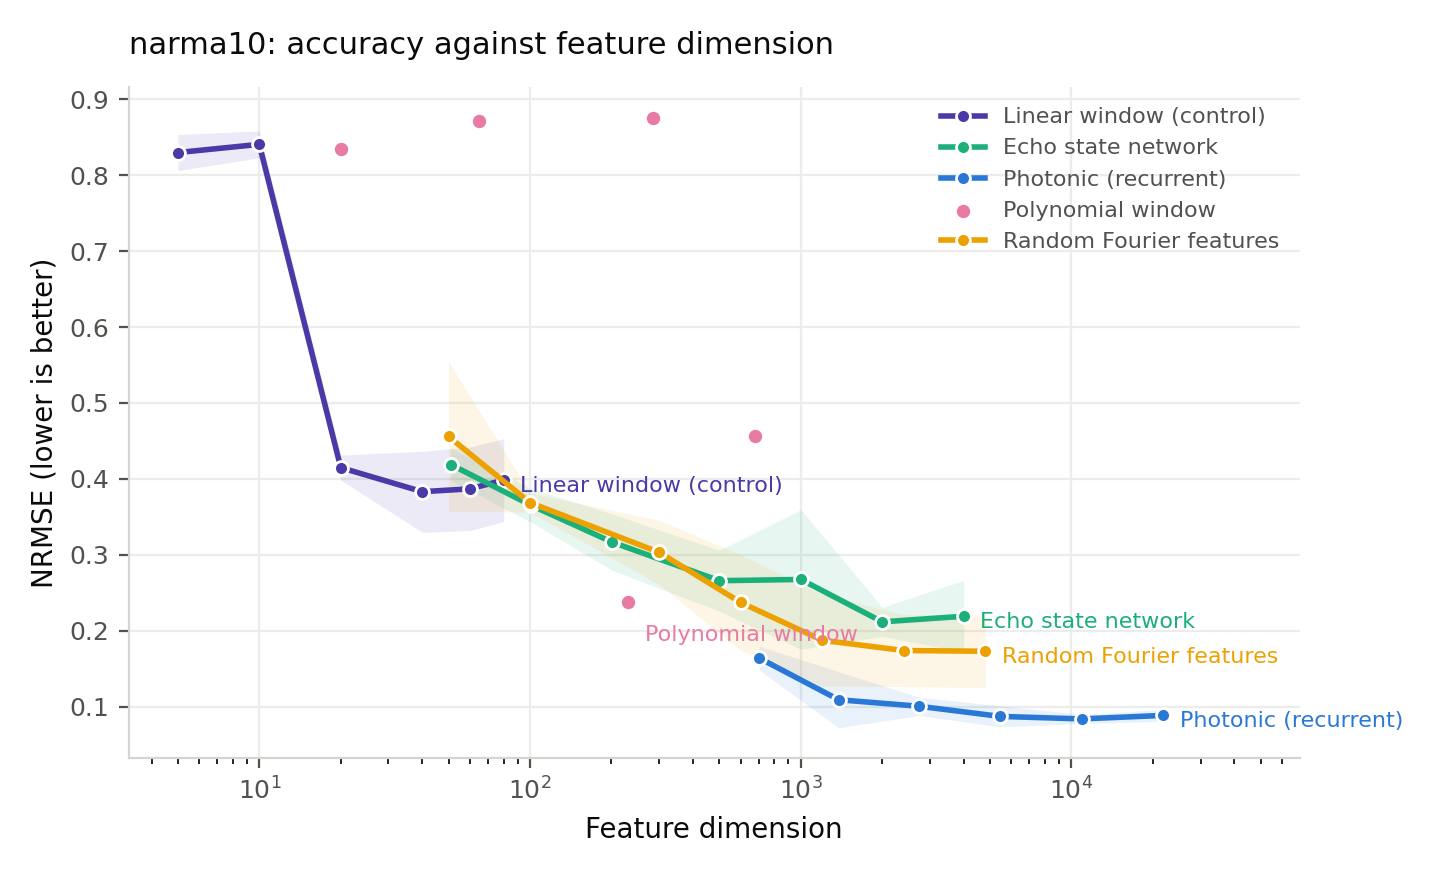
\includegraphics[width=0.86\textwidth]{capacity_narma10.png}
  \caption{NRMSE against feature dimension on NARMA-10. The echo state network saturates
           beyond $\sim\!2000$ units; the photonic map does not. A single photonic reservoir
           at 701 features already matches the echo state network's best.}
  \label{fig:capacity}
\end{figure}

\subsection{The encoding window tracks the task order}\label{sec:encoding}

NARMA-$N$'s target contains $u_t u_{t-N+1}$. A linear-optical map applies a unitary to an
encoding vector, so it can only form that product if both lags appear in the same encoding.
Sweeping the encoding window with everything else fixed gives optima of $8$, $12$ and $25$ for
NARMA-5, NARMA-10 and NARMA-20 respectively --- tracking the task order rather than being a
free-floating hyperparameter.

We note that in the small hardware-viable configuration used for that sweep, the feedback
contributes only $5$--$11\%$ and is slightly harmful on NARMA-5. The factor of two reported in
Section~\ref{sec:accuracy} is measured at the accuracy-tuned configuration. The benefit of
recurrence grows with model capacity, and we report both numbers.

\subsection{Memory and information processing capacity}\label{sec:ipc}

\begin{table}[H]\centering
  \PaperTableMemory
  \caption{Linear memory capacity \citep{jaeger2001esn} and information processing capacity
           \citep{dambre2012ipc} on i.i.d.\ uniform input, mean over 3 seeds.}
  \label{tab:memory}
\end{table}

The photonic map carries the highest information processing capacity \emph{per feature} but
substantially less linear memory than an echo state network. It trades memory depth for
nonlinearity, which is consistent with where it wins: NARMA targets are low-order polynomials
of a bounded stretch of history.

\subsection{Echo state property}\label{sec:esp}

Perturbing the initial state and driving two copies with identical input, the perturbation
decays for $g_{\text{fb}} \le 1.0$ and persists indefinitely for $g_{\text{fb}} \ge 1.5$. The
memory horizon lengthens with feedback gain --- 44, 72, 109 and 352 steps at
$g_{\text{fb}} = 0, 0.3, 0.6, 1.0$ --- and the best accuracy occurs just below the transition,
the standard edge-of-stability picture. All reported experiments use $g_{\text{fb}} = 0.3$,
inside the contracting regime.

\section{Robustness at measured hardware noise}\label{sec:noise}

Noise is simulated with Perceval's device model and threshold detectors, at operating points
read from Quandela's cloud API: Ascella at Hong--Ou--Mandel visibility $86.36\%$,
$g^{(2)}(0) = 1.95\%$, transmittance $2.44\%$, clock $80$\,MHz; Belenos at $82.7\%$, $18.2\%$
and clock $4.94$\,MHz. The configuration tested is the hardware-viable one --- two photons in
twelve modes --- not the accuracy-tuned configuration, which no current device could execute.

\begin{table}[H]\centering
  \PaperTableNoise
  \caption{Sensitivity to finite sampling (left), photon indistinguishability (centre) and
           multi-photon emission (right), NARMA-10.}
  \label{tab:noise}
\end{table}

\begin{figure}[H]\centering
  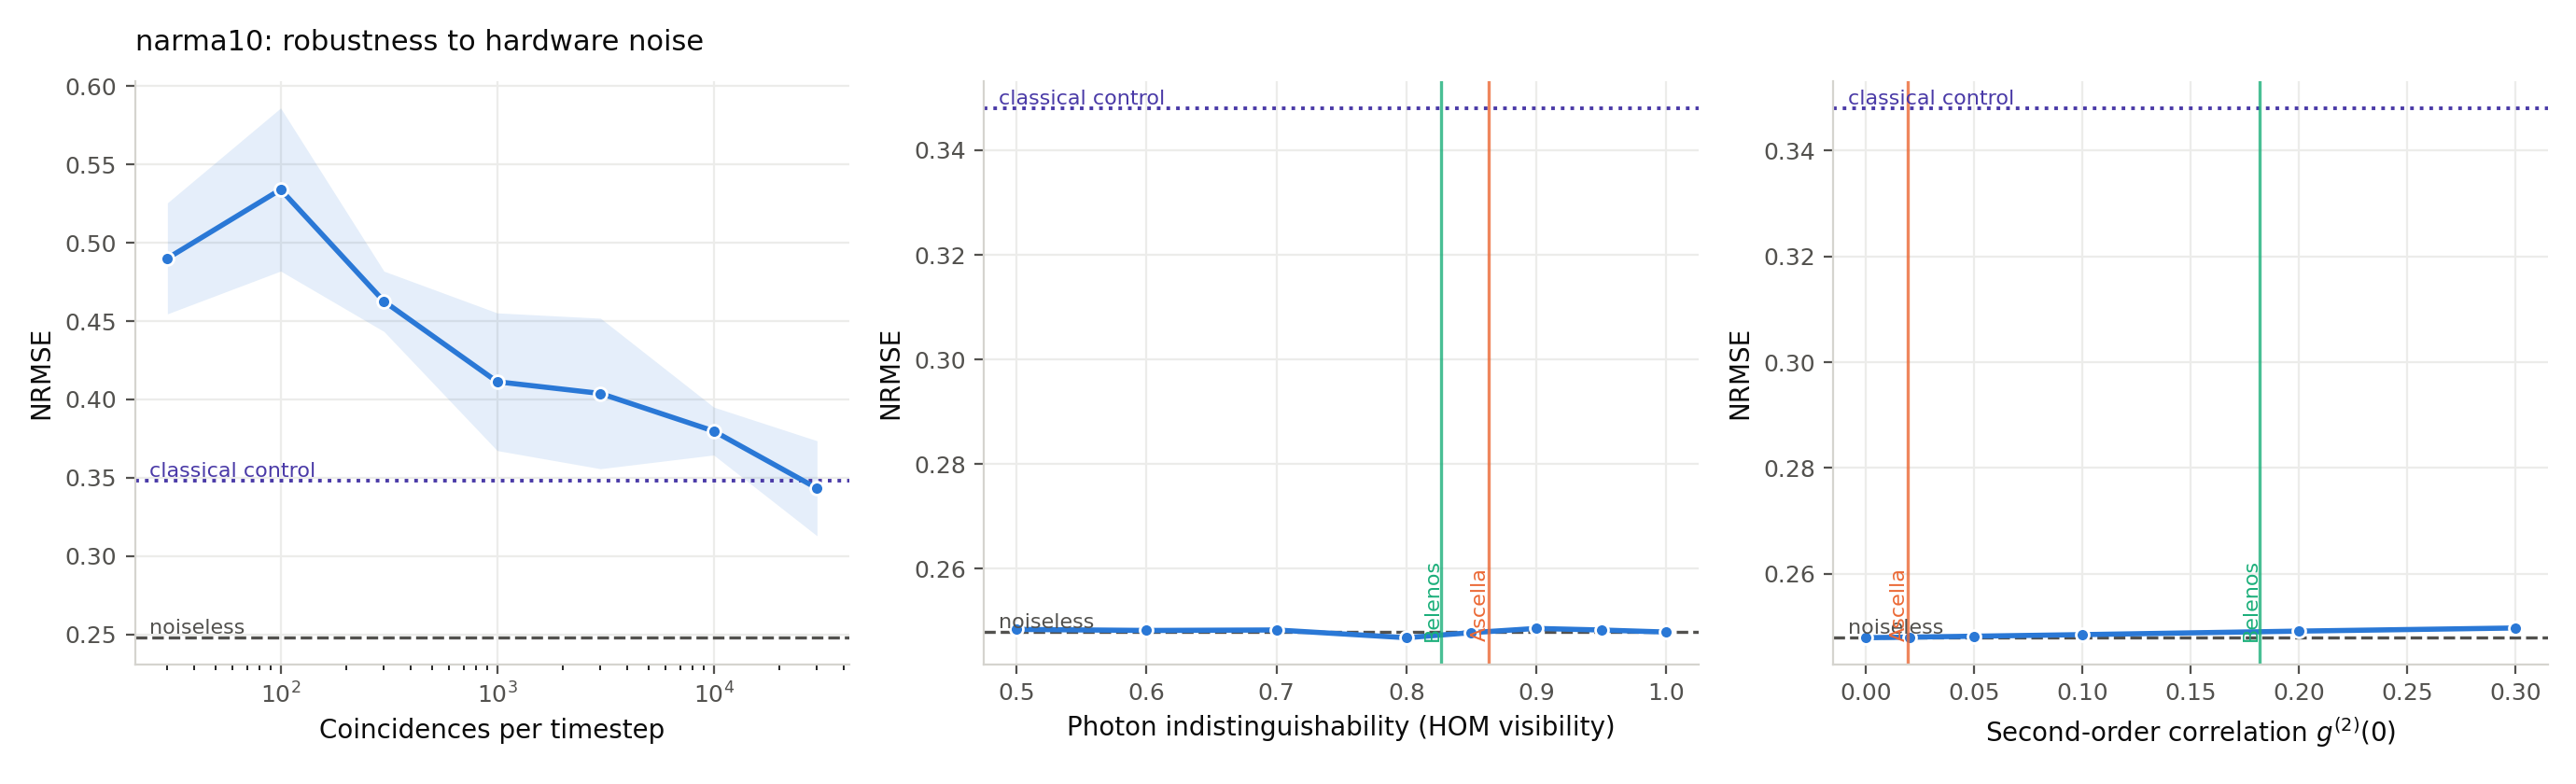
\includegraphics[width=\textwidth]{noise_narma10.png}
  \caption{Accuracy against each noise source. Dashed line: noiseless. Dotted line: the
           classical control. Vertical rules mark the measured Ascella and Belenos operating
           points, both well inside the flat region.}
  \label{fig:noise}
\end{figure}

Device imperfections are close to irrelevant. Accuracy is flat across
Hong--Ou--Mandel visibility from $0.50$ to $1.00$ and rises only $0.8\%$ as $g^{(2)}(0)$ goes
from $0$ to $0.30$. Running the full Ascella and Belenos models --- every source at once ---
gives $0.2483$ and $0.2465$ against a noiseless $0.2479$.

Finite sampling, by contrast, dominates. Extending the sweep to $10^{6}$ coincidences per
timestep gives NRMSE $0.418, 0.399, 0.321, 0.305, 0.285, 0.283$ at
$10^{3}, 10^{4}, 3\!\cdot\!10^{4}, 10^{5}, 3\!\cdot\!10^{5}, 10^{6}$ respectively, against
$0.275$ in the infinite-shot limit and $0.348$ for the classical control. Two thresholds
follow: roughly $3\!\cdot\!10^{4}$ coincidences per timestep are needed for the reservoir to
beat its classical control at all, and roughly $3\!\cdot\!10^{5}$ to come within $4\%$ of its
own noiseless limit, beyond which it is converged.

The asymmetry has a simple explanation. A reservoir is a random feature map, and the readout is
refitted on whatever map the device happens to realise; a slightly perturbed map is still a
perfectly good map, and imperfect indistinguishability merely interpolates towards the
distinguishable-particle distribution \citep{tichy2014distinguishability}, which is itself a
usable nonlinear feature map. Sampling noise is different in kind: it corrupts every feature
independently at every timestep and no readout can absorb it.

\subsection{Consequence: optimise rate, not photon quality}\label{sec:rate}

Detected $n$-fold coincidence rate scales as $\eta^{n}$ in the transmittance $\eta$, so photon
number is the dominant lever on the quantity that actually matters.

\begin{table}[H]\centering
  \PaperTableRates
  \caption{Coincidence rate and the time required to collect $3\!\times\!10^{4}$ events per
           timestep, at the measured operating points. Reaching the near-converged threshold
           of $3\!\times\!10^{5}$ costs ten times as long: $6.3$\,s per timestep at two
           photons on Ascella, against $4.3$ minutes at three.}
  \label{tab:rates}
\end{table}

\begin{figure}[H]\centering
  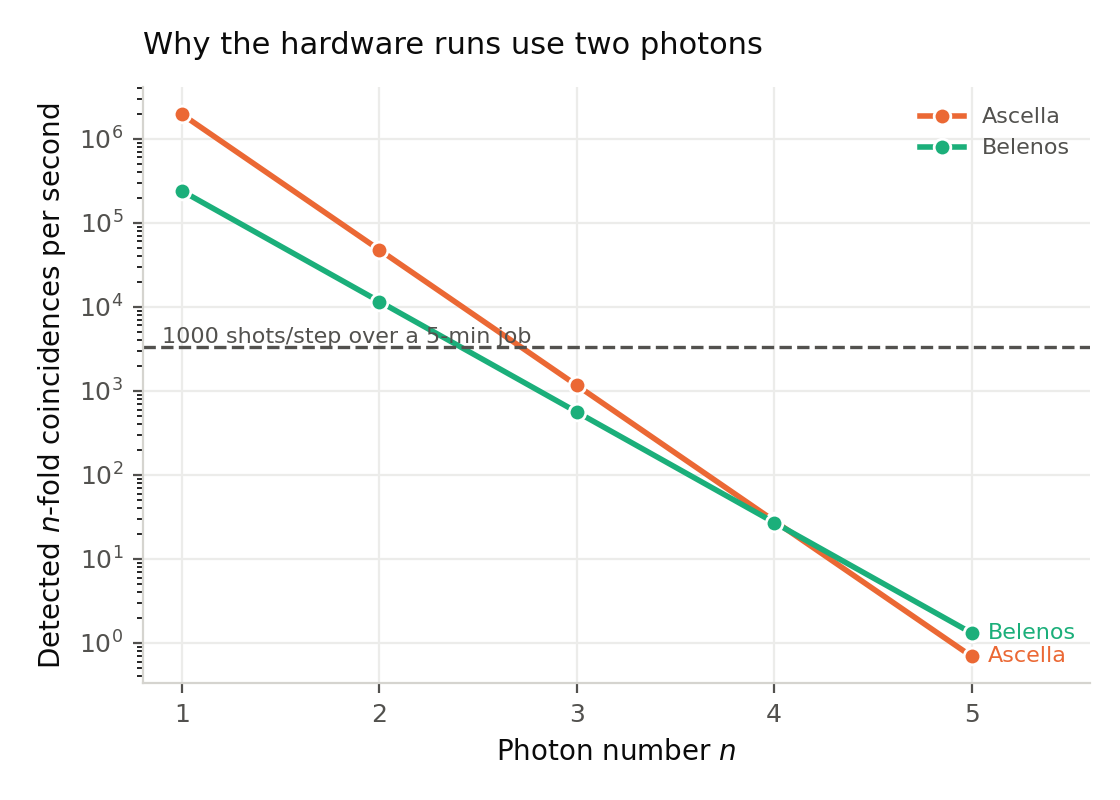
\includegraphics[width=0.62\textwidth]{coincidence_rate.png}
  \caption{Coincidence rate against photon number.}
  \label{fig:rate}
\end{figure}

This inverts the usual instinct that a quantum reservoir needs high-quality single photons. For
this class of model, two photons at high rate is strictly preferable to three at low rate. It
also explains a failed earlier attempt of our own: a three-photon probe on Belenos returned
$\sim\!48$ counts from 1000 requested shots spread over 56 Fock bins, and its features
correlated only $0.18$--$0.48$ with simulation. That was sampling noise, not a calibration
fault.

\section{Is it the interference, or a random nonlinear map?}\label{sec:quantumness}

Random Fourier features come close to this model on several tasks, so the question that decides
whether ``photonic'' is load-bearing is not whether a random nonlinear map helps --- it plainly
does --- but whether the \emph{interference} contributes. Partial distinguishability answers it
cleanly, because it interpolates exactly between the two hypotheses at otherwise identical
circuit, phases, shot count and readout. At $\mathcal{I} = 0$ the photons are classical
distinguishable particles and the distribution is the permanent of $|U|^2$, a positive matrix
and a classical stochastic feature map. At $\mathcal{I} = 1$ they are indistinguishable bosons
and the distribution is $|\mathrm{perm}(U)|^2$, with interference among the $n!$ assignments.

We evaluate in the infinite-shot limit so sampling cannot mask the effect, pair observations
across seeds (a seed fixes both the circuit draw and the data), and require an effect to clear
both $p < 0.05$ and half a seed standard deviation before calling it an effect.

\begin{table}[H]\centering
  \small
  \begin{tabular}{lrrrrrl}
    \toprule
    Task & $n$ & $\mathcal{I}{=}0$ & $\mathcal{I}{=}1$ & ratio & $p$ & verdict \\
    \midrule
    channel-eq & 2 & 0.1726 & 0.1728 & 0.999 & 0.571 & no detectable effect \\
    channel-eq & 3 & 0.1725 & 0.1737 & 0.993 & 0.541 & no detectable effect \\
    NARMA-10   & 2 & 0.2465 & 0.2373 & 1.039 & 0.886 & no detectable effect \\
    NARMA-10   & 3 & 0.2225 & 0.2198 & 1.012 & 0.280 & no detectable effect \\
    parity     & 2 & 0.7506 & 0.7901 & 0.950 & 0.324 & no detectable effect \\
    parity     & 3 & 0.3140 & 0.3835 & 0.819 & 0.166 & no detectable effect \\
    Henon      & 2 & 0.8811 & 0.8830 & 0.998 & 0.571 & no detectable effect \\
    Henon      & 3 & 0.8811 & 0.8849 & 0.996 & 0.034 & interference \emph{hurts} \\
    \bottomrule
  \end{tabular}
  \caption{Effect of photon indistinguishability, median NRMSE over 3 seeds. Seven of eight
           configurations show no detectable effect; ratios scatter in both directions and the
           one significant case is adverse.}
  \label{tab:quantumness}
\end{table}

We therefore state plainly that \textbf{this architecture is a classical random nonlinear
feature map realised in optics}. The interferometer and Fock measurement supply a useful
high-dimensional map; the indistinguishability of the photons is not what makes it work.

One distinction in Table~\ref{tab:quantumness} matters. On the parity task \emph{photon number}
helps substantially --- $n=3$ reaches $0.314$ against $n=2$'s $0.751$ --- while
indistinguishability does not. The resource being exploited is Fock-space dimension
$\binom{m}{n}$, not interference.

Two consequences follow. Scientifically, this explains Section~\ref{sec:noise}: insensitivity
to Hong--Ou--Mandel visibility there and the absence of an interference effect here are the same
fact observed twice. Practically, it lowers the hardware requirement, because a source for this
application need not be indistinguishable --- and HOM visibility, normally the headline figure
of merit for a single-photon source, is not the specification to optimise. Transmittance is
(Section~\ref{sec:crossover}).

\section{When would photonics beat simulating it?}\label{sec:crossover}

The obvious objection to a photonic reservoir at these scales is that a laptop simulates it
faster, and it deserves a number rather than a deflection. Classical simulation cost grows
combinatorially in photon number: composing the unitary costs $O(d m^3)$ and the permanent
batch costs $\binom{m}{n} \cdot n! \cdot n$ multiply-adds per timestep. The device's cost grows
as $1/\eta^{n}$, since it must accumulate a fixed number of coincidences and the rate falls as
$\eta^{n}$. Which grows faster settles the question.

Taking the measured throughput of our implementation ($7.3 \times 10^{7}$ complex multiply-adds
per second, single core) and the measured platform specifications, at the
$3 \times 10^{4}$-coincidence threshold established in Section~\ref{sec:noise}:

\begin{table}[H]\centering
  \PaperTableRates
  \caption{Coincidence rate and the time to collect $3\!\times\!10^{4}$ events per timestep.}
  \label{tab:rates2}
\end{table}

\textbf{There is no crossover at any photon number on current hardware.} The device is closest
at $n = 2$ and is still $1.6 \times 10^{3}$ times slower than simulating it on one core for
Ascella, and $6.6 \times 10^{3}$ times slower for Belenos.

The useful part is that the requirement is now quantitative. A crossover at $n = 12$ in $24$
modes would need $\eta \ge 0.105$ on Ascella against its present $0.0244$, a factor of four,
or $\eta \ge 0.132$ on Belenos, a factor of three. The required transmittance \emph{falls} with
photon number --- $0.978$ at $n=2$ down to $0.105$ at $n=12$ --- because classical cost
outgrows the rate penalty. High photon number is therefore the regime where optics could win,
provided loss drops far enough to reach it. At $n = 2$ and $n = 3$ on Belenos the required
transmittance exceeds unity, meaning simulation is so cheap there that no device could beat it.

This is why we make no computational-advantage claim, and why we read loss reduction rather
than photon count as the operative engineering target for this class of model.

\section{Hardware execution}\label{sec:hardware}

\textbf{No result in this paper is a measurement on a quantum processor.} Both
\texttt{qpu:ascella} and \texttt{qpu:belenos} reported \texttt{maintenance} throughout this
work.

The execution path itself has been run end to end on Quandela's cloud, including chunked
submission, threshold-detector sampling, coincidence post-selection and result caching. Over
600 timesteps at $8\!\times\!10^{3}$ requested coincidences per step, device-measured features
correlate with simulation at $0.999$ (worst case $0.994$). This is the quantitative validation
of the two-photon decision: the earlier three-photon probe on the Belenos QPU reached only
$0.18$--$0.48$, because at $\eta^{3}$ it collected $\sim\!48$ counts per step across 56 Fock
bins.

Quandela's cloud emulator platforms also corroborate Section~\ref{sec:noise} independently.
Submitting 30 identical phase settings to each platform at $2\!\times\!10^{4}$ shots and
measuring total variation against an exact local calculation gives $0.0211$ for the noiseless
\texttt{sim:slos} and $0.0288$ for \texttt{sim:ascella}, against $0.0193 \pm 0.0004$ for a
perfect multinomial sampler at that shot count --- a $+26\sigma$ excess for the emulator. The
device model is therefore real but small: it displaces the distribution by $0.008$ on top of a
sampling error of $0.019$. That is the same ordering Perceval's device model gives, reached
independently through Quandela's own emulator.

We note that the downstream NRMSE ordering is not evidence on this point in either direction:
\texttt{sim:ascella} scored better than the noiseless \texttt{sim:slos} in the 600-step run,
which is seed-to-seed scatter in a regression rather than a statement about the underlying
distributions. Only the distribution comparison settles it.

Because a closed feedback loop cannot be batched into a single cloud job
(Section~\ref{sec:free-feedback}), two protocols are provided. In \emph{replay}, the recurrence
is evaluated in simulation to produce the phase trajectory, which is then replayed on the
device as one batched job and the readout trained on device-measured features; this measures
the device's feature map faithfully but the feedback path is simulated, and we report it
as such. In \emph{open-loop}, feedback is disabled and every timestep is independent, so the run
is end-to-end on the device at the cost of a weaker model.

In practice the open-loop protocol is both the stronger claim and the better result: over 600
timesteps it reaches NRMSE $0.347$ against $0.393$ for replay and $0.423$ for the classical
control, a lift of $1.22$. This is consistent with Section~\ref{sec:encoding}, where the
feedback contributes little in the small hardware-viable configuration. Giving it up therefore
costs almost nothing at the scale a current device can run, while removing the only caveat the
replay protocol carries --- a useful result for anyone planning a hardware demonstration.

Two operational findings are worth recording for others attempting this. On the free tier a
job is cancelled at five minutes: one of our submissions was terminated at 307\,s having
completed 4\% of its iterations, which forces chunked submission with per-chunk caching. And
the shot budget per call must be set explicitly and generously, since the post-selection that
follows consumes it.

\section{Limitations}\label{sec:limitations}

\textbf{Everything here is simulated.} We claim no quantum advantage. The comparison is between
feature maps on classical data, and a passive interferometer is a classically simulable device
at these photon numbers by construction.

\textbf{Interference does not contribute.} Section~\ref{sec:quantumness} tests this directly
and finds no detectable effect on seven of eight configurations. Readers should treat this as a
result about the architecture rather than a caveat: what the optics supplies is a
high-dimensional random nonlinear map, and the useful resource is Fock-space dimension.

\textbf{No computational crossover.} Section~\ref{sec:crossover} shows the device is at best
$1.6\times10^{3}$ times slower than simulating it on one core, at any photon number, on current
hardware.

\textbf{A negative result on the financial task.} On S\&P~500 realised volatility the model
does not win and nothing is statistically distinguishable. We include the task because it was
pre-registered, and we draw no conclusion from it.

\textbf{A negative result on the predecessor architecture.} An earlier version of this work
used the same optics without recurrence, encoding a sliding window directly as phases. It did
not outperform a ridge regression on the raw window (MSE $5.38\!\cdot\!10^{-3}$ against
$5.24\!\cdot\!10^{-3}$ on NARMA-10), and no setting of encoding gain, circuit depth, photon
number or mode count changed that. The cause was an encoding that spanned only $0.58$ radians
of the available $2\pi$, leaving the optical features with $16\times$ less variance than the
classical block beside them. We report this because the failure mode is easy to reproduce and
hard to detect without a classical control in the table.

\textbf{Feature dimension.} The tuned configuration uses more features than the baselines.
Section~\ref{sec:capacity} is the honest version of Table~\ref{tab:benchmarks}, and any claim
should be read against it.

\textbf{Statistical power.} With 200--600 test points the Model Confidence Set does not
discriminate. Our conclusions rest on Diebold--Mariano tests.

\section{Conclusion}\label{sec:conclusion}

Feeding a leaky-integrated state back into the phase encoding of a fixed interferometer turns a
windowed optical feature map into a reservoir, and does so at no additional photonic cost,
since the feedback is classical and happens between measurement batches. The resulting model
outperforms tuned classical feature maps on NARMA-10 and NARMA-20 at matched feature dimension,
ties on Mackey--Glass, and does not win on realised volatility.

For hardware, the operative result is that the model is insensitive to the imperfections
photonic platforms are usually characterised by, and limited instead by how many coincidences
can be collected. That converts a vague question about device quality into a concrete
engineering target, and suggests that the useful direction for this class of model is fewer
photons at higher rate.

\bibliographystyle{plainnat}
\bibliography{refs}

\end{document}
